\chapter{Datasets \& Transcribing}\label{ch:datasets}
\section{Datasets}
We use learning-based classification algorithms.
This means, given a set of rules, they try to induce the underlying patterns of a training set.
The resulting patterns are then used to classify unseen entities of a test set.
To train and test our algorithms we use two datasets, each consisting of labeled text pairs.
A pair has the label \textit{True} if both texts were authored by the same person and \textit{False} if not.\\\\
% PAN 2020 Fanfiction
First, we will use the small official dataset from the PAN 2020 task on Authorship Verification from \cite{bevendorff2020overview}.
This allows us to compare our results to the other methods submitted.
It consists of 52.601 text pairs collected from the fanfiction website \url{fanfiction.net}.
The dataset file is formatted in the PAN 2020 format with each line containing a json object with the text pair, an ID, and optionally some additional information such as the corresponding fandoms\footnote{The franchise a fanfiction text belongs to. It can be seen as the topical domain of the text.}.
In contrast, the large official dataset contains 256.000 samples.
This is roughly five (4.86) times as many samples as the small dataset.
Efforts have been made to maximally optimize the methods used, but due to certain implementation details, the utilization of the large Fanfiction dataset remains infeasible for now.\\
% Gutenberg
We source the second dataset from \cite{stein2019unbiasedGutenbergCorpus}.
It presents a dataset containing science fiction and adventure texts from the 19th and 20th century, compiled from books from Project Gutenberg\footnote{\url{https://www.gutenberg.org/}}.
As discussed earlier, the aim of this dataset is to reduce common biases in datasets for Authorship Verification.
This makes it a good candidate for evaluating new authorship verifiers.
With only 262 text pairs, it is much smaller than the first dataset used.
To maximally use the information in this dataset, we employ cross-validation in our evaluation instead of a standard train-test-split method.
This dataset is in the old format, used before PAN 2020, and is converted to the new PAN 2020 format for standardization\footnote{The code for the conversion is available at \url{https://github.com/av-pt/NAACL-19}}.\\

\begin{figure}
  \centering
  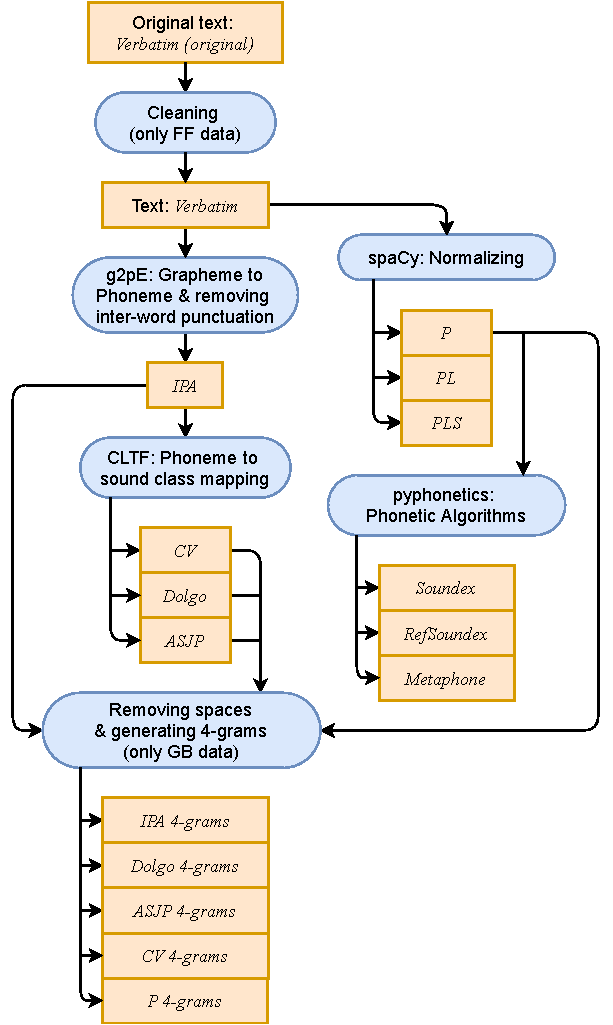
\includegraphics[width=0.7\textwidth]{figures/transcription}
  \caption{Transcription setup, orange = data, blue = process.}
  \label{fig:transcription}
\end{figure}


% Transcribing
\section{Transcribing}
We use a range of open-source libraries to transcribe the datasets.
Figure~\ref{fig:transcription} shows the process a given text undergoes during transcription.
Because the Fanfiction dataset is at times noisy and contains artifacts that are phonetically irrelevant (e.g., long punctuation sequences, HTML-tags), we clean it with the following steps:
\begin{enumerate}
  \item Remove tokens longer than 23 characters.\\
        $\rightarrow$ The longest token occuring in the Fanfiction dataset that also occurs in the ASPELL\footnote{\url{http://aspell.net/}} dictionary is 23 characters long. Longer tokens are mainly artifacts.
  \item Remove tokens with 3 or more punctuation symbols.\\
        $\rightarrow$ Tokens with many punctuation symbols are mainly artifacts.
  \item Remove tokens containing symbols that are \textit{not} in the following set:\\$\{symbol\ |\ isTranscribable(symbol) \land isPunctuation(symbol)\}$\\e.g. $\{a, b, c, \dots, \textipa{\~n}, \textipa{\"e}, \dots, !, ?, \texttt{"}, \dots\}$\\
        $\rightarrow$ Tokens with such non-transcibable symbols do not create meaningful transcriptions.
  \item Replace all double quotes with single quotes.\\
        $\rightarrow$ During the creation of the Fanfiction dataset all types of quotes were normalized to double quotes. This leads to combinations that are not transcribed correctly (e.g. ``I"m'' is erroneously transcribed to \textipa{[Im]} instead of \textipa{[aIm]}). On the other hand, single quotes used in place of double quotes do not present any difficulties in transcribing.
  \item Remove excessively long or short texts ($<20500$ and $\geq22500$ characters, around 1.6\% of the data).
\end{enumerate}
The actual transcription steps are the same for the texts from both datasets.
First, we transcribe a given text to \textit{IPA} using g2pE introduced by \cite{kyubyong2019g2pE}.
It works as follows:
\begin{enumerate}
    \item Expand numbers and currency symbols (e.g.,\ ``\$400'' to ``four hundred dollars'').
    \item Use part-of-speech information to find the correct pronunciations for heteronyms, i.e., for words that have multiple context-dependant pronunciations.
    \item Look up pronunciations in the Carnegie Mellon University Pronouncing Dictionary\footnote{\url{http://www.speech.cs.cmu.edu/cgi-bin/cmudict/}}.
    \item For out-of-vocabulary words use a neural net model to predict their correct pronunciations.
\end{enumerate}
We use this method over a simpler approach because it exploits word context to find the correct pronunciation.
Additionally, it creates \textit{IPA} representations \textipa{segmented} into phonemes.
This is important for the next step, generating the broader sound class transcriptions using the Cross-Linguistic Transcription Systems project by \cite{list2018cltsIntro}.
CLTS serves as a phoneme-by-phoneme mapping between different transcription and sound class systems.
Given a list of \textit{IPA} transcribed phonemes, they can be mapped to a range of other systems.
As words in \textit{IPA} can contain arbitrary supra-segmental letters, and it is hard to segment these words into phonemes after transcribing, \cite{list2018sequence} recommends using segmented IPA representations.
Transcribing, for example, the word ``make'' to \textit{IPA} results in \textipa{[meIk]}.
In contrast to other algorithms, g2pE produces the correct segmentation \textipa{[m eI k]}.
Using CLTS to convert this to the \textit{Dolgo} system we correctly get ``MVK''.
If we were, for example, to naively segment \textipa{[meIk]} to \textipa{[m e I k]} by interpreting each \textit{IPA} symbol as a phoneme, we would incorrectly get ``MVVK'' as a result for the \textit{Dolgo} system.
For the Gutenberg dataset, we also generate space separated character $4$-grams for the systems above.\\
Punctuation and stop word removal, as well as lemmatization is done with spaCy\footnote{\url{https://spacy.io/}} for speed and robustness.
For the punctuation-removed data (\textit{P}) we also create $4$-grams.
They can be used as a generic $n$-gram approach compared to $n$-gram approaches using transcriptions as the transcriptions above also have punctuation removed.
The other phonetic algorithms --- \textit{Soundex}, \textit{RefSoundex} and \textit{Metaphone} --- work with verbatim text on word level, i.e.,\ they do not use context but transcribe each word in isolation.
Thus, we space-tokenize the punctuation-removed data (\textit{P}) and use the resulting lists as input for these algorithms.
For the transcriptions themselves we use the library pyphonetics\footnote{\url{https://github.com/Lilykos/pyphonetics}}.
The source code in this library is based on Talisman.js\footnote{\url{https://yomguithereal.github.io/talisman/}} which itself is based on the Apache commons codec\footnote{\url{http://commons.apache.org/proper/commons-codec/userguide.html}}.
The source code for transcribing datasets formatted in the PAN 2020 standard is available on GitHub\footnote{\url{https://github.com/av-pt/ba-util}}.

\section{Transcription Characteristics}
To better understand the characteristics of the phonetic transcription systems and the idiosyncrasies of the datasets, we conduct some preliminary investigations.
We calculate the vocabulary size scaling factor (\textit{VSSF}) for each transcription system by determining the ratio of the number of distinct lexical types before and after transcribing.
A \textit{VSSF} of 1.5, for example, indicates that the examined transcription system increases the vocabulary size by 50\%.
This way, we can assess the granularity of the different transcription systems.
A vocabulary reduction of 50\%, for example, indicates that on average two words are binned into one transcription.
In practice, there may be some transcriptions grouping many words while many transcriptions would have a one-to-one mapping to a single word.
We calculate the absolute vocabulary size and the \textit{VSSF} per transcription system per dataset.
Table~\ref{tab:system_characteristics} shows the results.\\
\begin{table}
\caption{Effects of transcription systems on the vocabulary sizes of the datasets. \textit{Verbatim} represents plain English text. \textit{Verbatim (original)} is the uncleaned version of the Fanfiction dataset.}
\label{tab:system_characteristics}
\centering\small
\begin{tabular}{@{}l@{\hspace{1\tabcolsep}}rlrl@{}} % Use @{\hspace{2\tabcolsep}} to double the spacing
\toprule
\bf System & \bf \specialcell{GB\\absolute} & \bf \specialcell{GB\\VSSF} & \bf \specialcell{FF\\absolute} & \bf \specialcell{FF\\VSSF} \\
\midrule
\textit{Verbatim (orig.)} & -- & -- & 795621 & 1.0426 \\
\textit{IPA} & 60673 & 1.2068 & 782424 & 1.0253 \\
\textit{ASJP} & 55913 & 1.1121 & 691146 & 0.9057 \\
\textit{Verbatim} & 50277 & 1.0 & 763097 & 1.0 \\
\textit{P} & 50277 & 1.0 & 754293 & 0.9885 \\
\textit{PL} & 40924 & 0.814 & 739629 & 0.9692 \\
\textit{PLS} & 40704 & 0.8096 & 739530 & 0.9691 \\
\textit{Dolgo} & 36288 & 0.7218 & 384440 & 0.5038 \\
\textit{RefSoundex} & 29441 & 0.5856 & 229360 & 0.3006 \\
\textit{Metaphone} & 26501 & 0.5271 & 210973 & 0.2765 \\
\textit{Soundex} & 4250 & 0.0845 & 6471 & 0.0085 \\
\textit{CV} & 1954 & 0.0389 & 9436 & 0.0124 \\
\textit{IPA 4-grams} & 176092 & 3.5024 & -- & -- \\
\textit{P 4-grams} & 103983 & 2.0682 & -- & -- \\
\textit{ASJP 4-grams} & 78246 & 1.5563 & -- & -- \\
\textit{Dolgo 4-grams} & 4061 & 0.0808 & -- & -- \\
\textit{CV 4-grams} & 16 & 0.0003 & -- & -- \\
\bottomrule
\end{tabular}
\end{table}
\begin{figure}
  \centering
  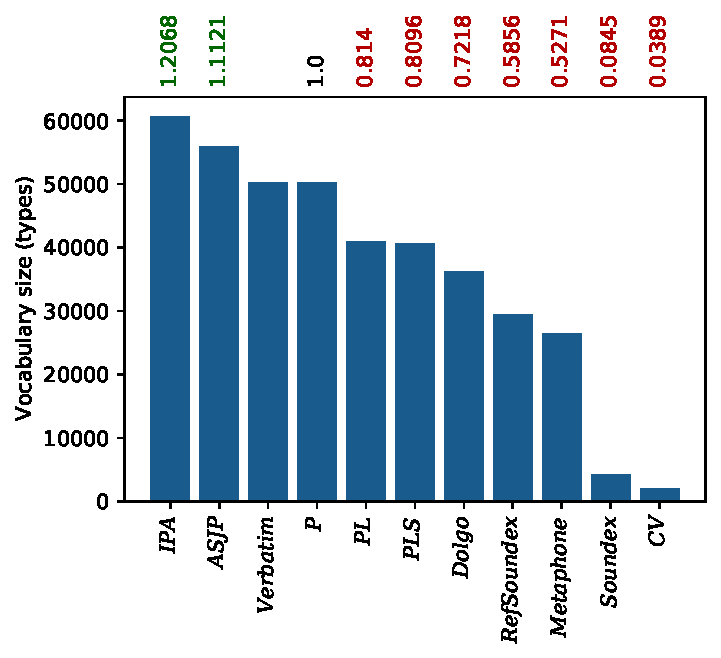
\includegraphics[width=0.7\textwidth]{figures/vocab_sizes_2021-07-28_14-42-08_gb_pt}
  \caption{Vocabulary sizes for transcriptions on Gutenberg dataset with \textit{VSSF}s above.}
  \label{fig:vssf_transcriptions_gb}
\end{figure}
First, let us take a look at findings for the Gutenberg dataset, which are visualized in figure~\ref{fig:vssf_transcriptions_gb}.
The \textit{verbatim} text contains 50277 types.
Both \textit{IPA} and \textit{ASJP} increase the vocabulary size by a significant amount, 20.68\% and 11.21\% respectively.
This is to be expected as the alphabet of both systems is larger than the alphabet of \textit{verbatim} text and thus more types can be generated.
The text with removed punctuation (\textit{P}) retains the same amount of types as \textit{verbatim} text because punctuation symbols are not counted towards the vocabulary size.
By further lemmatizing the texts (\textit{PL}), more tokens are binned and the resulting vocabulary is reduced by 18.6\%.
Eliminating stop words (\textit{PLS}) removes 220 more types.
The \textit{Dolgo} system has an even smaller amount of types, but still retains more type granularity than the more simple phonetic algorithms.
\textit{RefSoundex} and \textit{Metaphone} reduce the vocabulary size by 41.44\% and 47.29\% respectively.
Because of its length restriction to four characters, \textit{Soundex} can at most produce 8,918 unique types (A000 to Z666) with only 4250 of them appearing in the data.
Lastly, \textit{CV} reduces the number of types the most and retains only 1954 types.
A reduction to 3.89\% of the original vocabulary size implies that on average ca.\ 26 words are binned into one transcription.\\
\begin{figure}
  \centering
  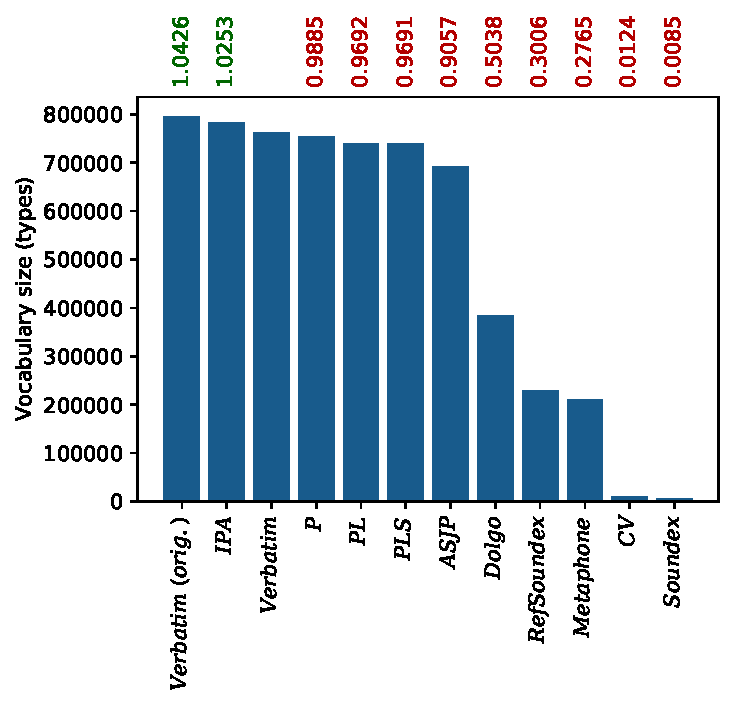
\includegraphics[width=0.7\textwidth]{figures/vocab_sizes_2021-07-27_16-57-38_ff_pt}
  \caption{Vocabulary sizes for transcriptions on Fanfiction dataset with \textit{VSSF}s above.}
  \label{fig:vssf_transcriptions_ff}
\end{figure}
Figure~\ref{fig:vssf_transcriptions_ff} shows the results for the same analysis but using the Fanfiction dataset.
Both plots are predominantly similar but exhibit a few interesting differences stemming from the characteristics of the transcription systems and the datasets.
Note that the Fanfiction dataset is substantially larger than the Gutenberg dataset, also leading to a larger total vocabulary count.\\
First, the vocabulary size of the uncleaned (original) \textit{verbatim} text is 4.26\% larger than that of the cleaned one.
This was expected as we removed certain words during cleaning.
Next, it can be observed that there is a difference between \textit{verbatim} text and punctuation-removed text (\textit{P}).
This may stem from the Fanfiction dataset including many more different punctuation symbols which are removed to create the \textit{P} transcription but not when counting types in \textit{verbatim} text.
Also, the relative difference between \textit{P} on the one hand and \textit{PL} as well as \textit{PLS} on the other is much smaller.
This could indicate that the Fanfiction dataset has many out-of-vocabulary tokens that are not easily lemmatized.
Compared to the Gutenberg dataset, which consists of texts from published books, this would make sense as the acceptance criteria for Fanfiction stories are much lower than those for books.
For the phonetic algorithms, \textit{Soundex} has a smaller vocabulary than \textit{CV}.
As mentioned above, the codes generated by the \textit{Soundex} algorithm are bound to 4 characters in length.
Because \textit{CV} tokens are only restricted to a binary alphabet, but do not have any length restrictions, with a large enough text sample the \textit{CV} vocabulary outnumbers the \textit{Soundex} vocabulary.
To substantiate this claim, we created a vocabulary list for each text pair in the Fanfiction dataset.
Then we accumulated the vocabulary lists one by one to examine if the transcribed texts follow Heaps' Law as defined in \cite{schutze2008introduction}.
\begin{figure}
  \centering
  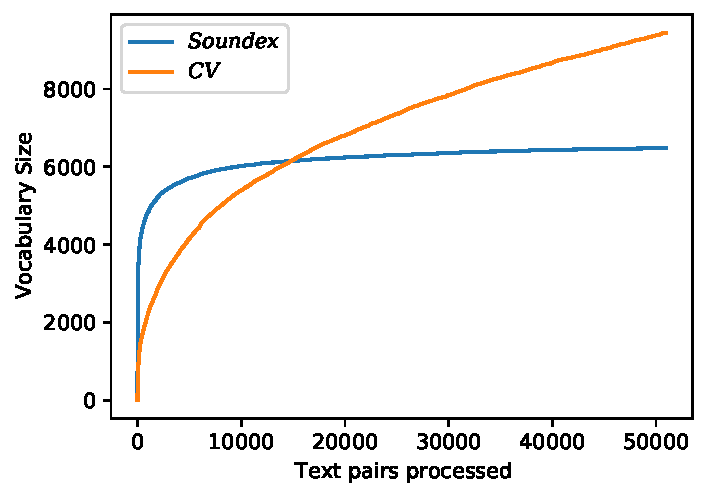
\includegraphics[width=0.7\textwidth]{figures/cum_vocab_size_ff_shuffled_soundexcv}
  \caption{Accumulated vocabulary size for \textit{Soundex} and \textit{CV}, shuffled Fanfiction dataset.}
  \label{fig:cumvocab_soundexcv}
\end{figure}
Figure~\ref{fig:cumvocab_soundexcv} shows the sizes for the accumulated vocabulary for \textit{Soundex} and \textit{CV} when reading in the texts from the Fanfiction dataset in a shuffled order.
The vocabulary of the \textit{Soundex} transcription grows fast in the beginning but then begins to max out at around 6000 types.
For the \textit{CV} transcription on the other hand, the accumulated vocabulary size grows slowly in the beginning, probably due to its restricted alphabet, but does not hit a ceiling and continues to grow beyond \textit{Soundex}'s vocabulary size.\\
Arguably, the most notable difference is that when transcribing the Gutenberg dataset \textit{ASJP} leads to an increase in vocabulary size whereas using the Fanfiction dataset \textit{ASJP} surprisingly results in a significant reduction of the vocabulary.
Note that as shown in figure~\ref{fig:transcription} \textit{ASJP} results from the \textit{IPA} transcription.
To attain a clearer view of what is happening here, we also calculate the accumulated vocabulary sizes for \textit{Verbatim}, \textit{IPA}, \textit{ASJP}, and \textit{Dolgo}, shown in figure~\ref{fig:cumvocab_all}.
\begin{figure}
  \centering
  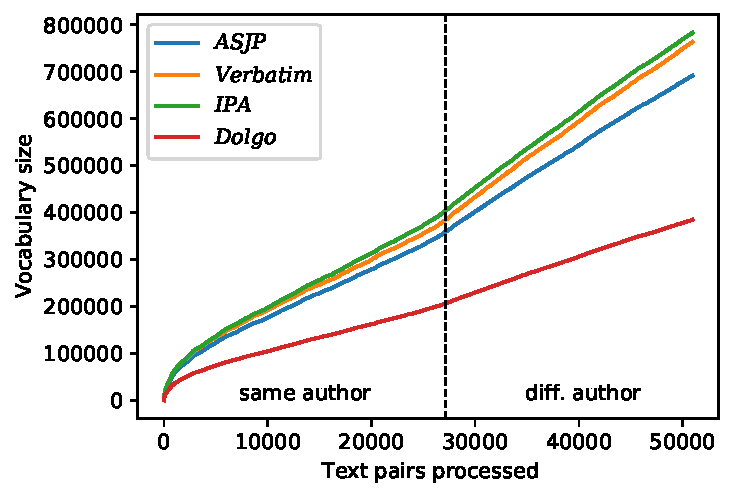
\includegraphics[width=0.7\textwidth]{figures/cum_vocab_size_ff_inorder_all}
  \caption{Accumulated vocabulary size for \textit{Verbatim}, \textit{IPA}, \textit{ASJP}, and \textit{Dolgo}, in-order Fanfiction dataset.}
  \label{fig:cumvocab_all}
\end{figure}
This plot poses two additional questions\footnote{Both phenomena persist when using single texts instead of text pairs for the cumulative vocabulary size analysis.}:
\begin{enumerate}
    \item Why is there a sudden change in slope in the accumulated vocabulary size?
    \item Why do \textit{IPA} and \textit{verbatim} text diverge on the left side but stay at a constant difference after the change in slope on the right side?
\end{enumerate}
The first question has an obvious answer.
The Fanfiction dataset is sorted.
The first half consists of only same-author pairs with all different-author pairs residing in the second half.
\begin{table}
\caption{Author distribution of the datasets used.}
\label{tab:dataset_authors}
\centering\small
\begin{tabular}{@{}l@{\hspace{1\tabcolsep}}lll@{}} % Use @{\hspace{2\tabcolsep}} to double the spacing
\toprule
\bf  & \bf Gutenberg & \bf Fanfiction \\
\midrule
No. of authors in same-author part & 54 & 6397 \\
No. of authors in different-author part & 56 & 47813 \\
No. of authors in both parts & 53 & 1555 \\
Texts per author in same-author part & 4.8148 & 8.7022 \\
Texts per author in diff-author part & 4.7143 & 1.036 \\
\bottomrule
\end{tabular}
\end{table}
Table~\ref{tab:dataset_authors} shows information on the author distribution of both datasets segmented into same-author and different-author parts.
With 47813 authors, the different-author part of the Fanfiction dataset has around 7.47 times as many authors as the same-author part.
For the same-author part, one author wrote 1.036 individual texts on average whereas for the different-author part this number is 8.7022\footnote{Or in terms of dataset samples, on average authors contributed to 0.518 and 4.3511 text pairs respectively.}.
It comes as no surprise then that --- despite individual text and vocabulary sizes being nearly equal for both parts --- the vocabulary of the different-author part is much more diverse.
This diversity leads to the higher slope in the different-author part.
As a side note, the bias-mitigated Gutenberg dataset does not exhibit a change of slope when analyzing it as above.
This is also reflected in the number of authors for the same- and different-author parts in table~\ref{tab:dataset_authors}.
The number of authors for both parts are almost identical, and most authors appear in both parts.
Also, the number of texts an author contributed to the dataset is nearly equal between both parts.
We conclude that the number of authors is correlated to the vocabulary size of a given dataset.
Further investigations are necessary to determine whether the difference in author distribution and thus in vocabulary size in the Fanfiction dataset has an effect on the results from the PAN 2020 task where this dataset was used.\\
\begin{figure}
  \centering
  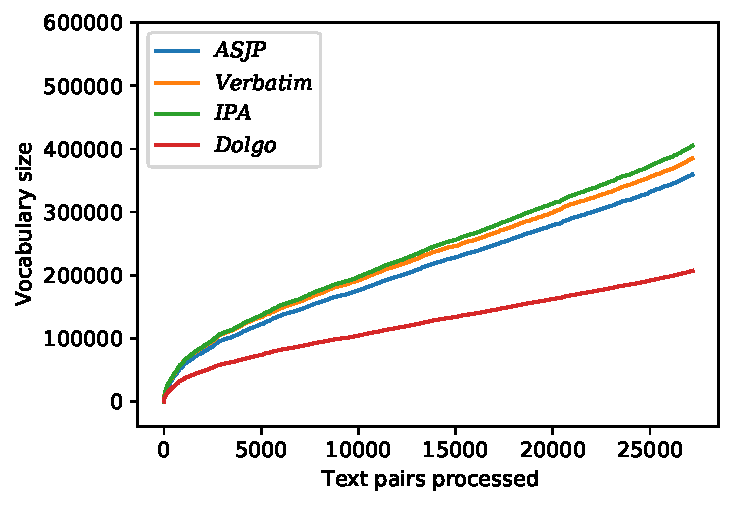
\includegraphics[width=0.7\textwidth]{figures/cum_vocab_size_ff_inorder_onlysame_ipa}
  \caption{Same-author part of accumulated vocabulary size for \textit{Verbatim}, \textit{IPA}, \textit{ASJP}, and \textit{Dolgo}, in-order Fanfiction dataset.}
  \label{fig:cumvocab_same}
\end{figure}
\begin{figure}
  \centering
  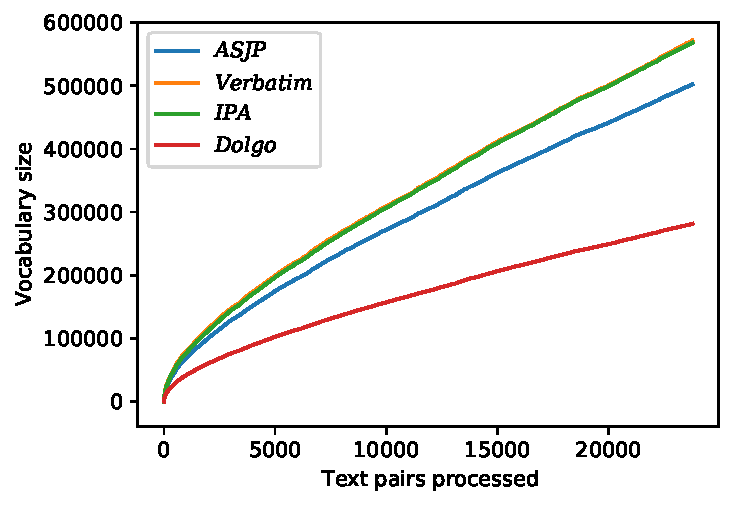
\includegraphics[width=0.7\textwidth]{figures/cum_vocab_size_ff_inorder_onlydiff_ipa}
  \caption{Different-author part of accumulated vocabulary size for \textit{Verbatim}, \textit{IPA}, \textit{ASJP}, and \textit{Dolgo}, in-order Fanfiction dataset.}
  \label{fig:cumvocab_diff}
\end{figure}
As of yet, we do not have an answer to the second question.
To change the perspective of this phenomenon, figures~\ref{fig:cumvocab_same} and~\ref{fig:cumvocab_diff} show the cumulative vocabulary size for the same-author and different-author part in isolation.
As expected, all curves follow Heaps' Law and the total vocabulary of the same-author part is lower than that of the different-author part.
The surprising difference is that the curves for \textit{Verbatim} and \textit{IPA} in figure~\ref{fig:cumvocab_diff} do not diverge.
In contrast to the same-author part, for the different-author part the transcription to \textit{IPA} does \textit{not} lead to an increased vocabulary size.
We investigated some possible explanations of this phenomenon.
The samples from both parts are transcribed in one coherent process and also plotted in one go, lowering the probability of an implementation error.
The percentage of alphabet characters (a-z, A-Z) in both parts is almost equal.
The only small difference we found is in the fraction of words that occur in the ASPELL dictionary.
For the same-author part 15\% of the words are in ASPELL while for the different-author part only 10\% are in ASPELL\@.\\
We suspect that the decrease in vocabulary size of \textit{ASJP} compared to \textit{verbatim} text (fig.~\ref{fig:vssf_transcriptions_ff}) has two reasons.
First, the missing increase for the vocabulary size of \textit{IPA} in the different-author part.
As \textit{IPA} is the transcription preceding \textit{ASJP}, the vocabulary size of the former directly impacts the that of the latter.
Second, in figure~\ref{fig:cumvocab_same} we observe that \textit{ASJP} still produces a lower vocabulary count, even for the same-author part only.
This lets us speculate that some other factor, e.g., the quality of the dataset, must also play a roll in its transcription.
Maybe both, the same-author and the different-author part, are affected by the same phenomenon with the same-author part affected only slightly.
This hypothesis could be supported by comparing the vocabulary increase of \textit{IPA} between both datasets.
With the Gutenberg dataset, \textit{IPA} increases the vocabulary by 20.68\% (fig.~\ref{fig:vssf_transcriptions_gb}) while with the Fanfiction dataset the vocabulary is only increased by 2.53\% (fig.~\ref{fig:vssf_transcriptions_ff}).
Still, this comparison should be interpreted cautiously because of the bespoken size differences of the datasets.
To this end, further investigation is needed.\\
\begin{figure}
  \centering
  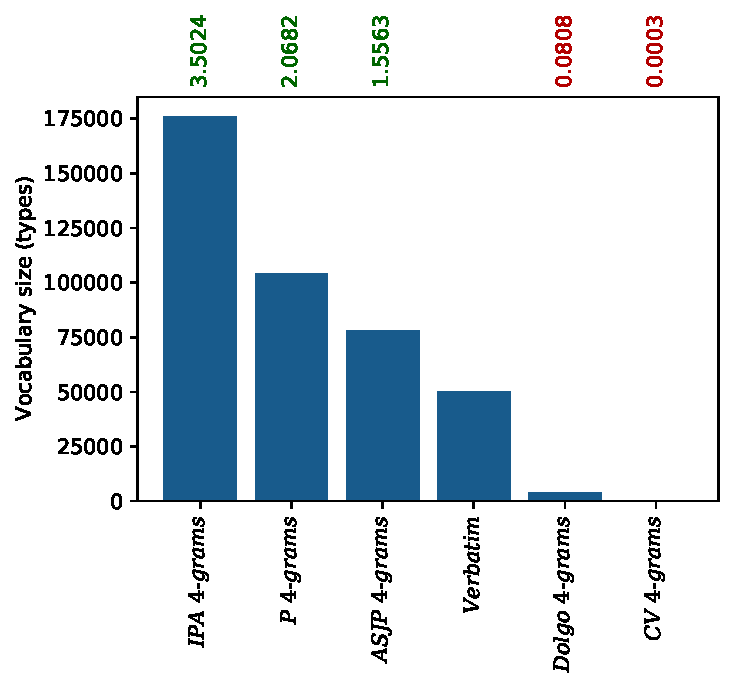
\includegraphics[width=0.7\textwidth]{figures/vocab_sizes_2021-07-28_14-42-08_gb_ngram}
  \caption{Vocabulary sizes for $4$-grams compared to \textit{Verbatim}.}
  \label{fig:vssf_ngrams_gb}
\end{figure}
Figure~\ref{fig:vssf_ngrams_gb} shows the vocabulary sizes for the $4$-grams, i.e., the amount of unique $4$-grams generated from each transcription of the Gutenberg dataset, compared to the vocabulary size of \textit{verbatim} text.
With a binary alphabet, \textit{CV} creates only 16 unique $4$-grams.
This is followed by \textit{Dolgo}, which could at most create 20736 $4$-grams of which 4061 appear in the data.
\textit{ASJP} increases upon the vocabulary count of \textit{verbatim} text, as it has a bigger alphabet.
The $4$-grams generated from punctuation-removed text have an even higher count.
This is due to intra-word punctuation not being removed and thus retaining many of the punctuation symbols from \textit{verbatim} text.
Lastly, \textit{IPA} generates by far the most $4$-grams, as it has the biggest alphabet of all transcriptions used.